% ------------------------------------------------------------------------------
% TYPO3 Version 10.4 - What's New (English Version)
%
% @author	Michael Schams <schams.net>
% @license	Creative Commons BY-NC-SA 3.0
% @link		https://typo3.org/help/documentation/whats-new/
% @language	English
% ------------------------------------------------------------------------------

\section{Changes for Integrators}
\begin{frame}[fragile]
	\frametitle{Changes for Integrators}

	\begin{center}\huge{Chapter 2:}\end{center}
	\begin{center}\huge{\color{typo3darkgrey}\textbf{Changes for Integrators}}\end{center}

\end{frame}

% ------------------------------------------------------------------------------
% Feature | 89513 | Provide password recovery for backend users

\begin{frame}[fragile]
	\frametitle{Changes for Integrators}
	\framesubtitle{Password Recovery Email (1)}

	\begin{itemize}

		\item Password resets for backend users are only valid for 4 hours.\newline
			This time limit is not configurable.
		\item To strengthen security, the function can be disabled for admin users or for all users.
		\item If users share one email address, an alternative email text is used.
		\item TCA field \texttt{be\_users.email} must not be set to \texttt{eval=email}.

		\item The function only works for users, who:
			\begin{itemize}
				\item have an email address set,
				\item have a password set, and
				\item are not disabled/deleted.
			\end{itemize}

	\end{itemize}

\end{frame}

% ------------------------------------------------------------------------------
% Feature | 89513 | Provide password recovery for backend users

\begin{frame}[fragile]
	\frametitle{Changes for Integrators}
	\framesubtitle{Password Recovery Email (2)}

	\begin{itemize}
		\item Password recovery emails can also be triggered on the command line.
	\end{itemize}

	\begin{figure}
		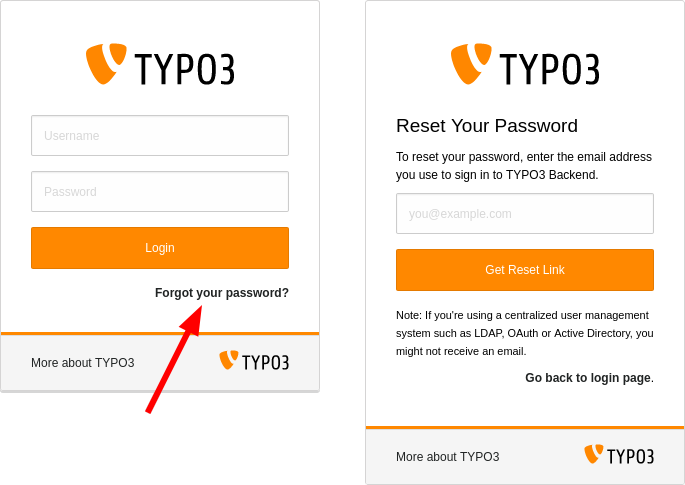
\includegraphics[width=0.9\linewidth]{ChangesForIntegrators/89513-ProvidePasswordRecoveryForBackendUsers.png}
	\end{figure}

\end{frame}

% ------------------------------------------------------------------------------
% Important | 90285 | Fresh installs without constraint for typo3fluid/fluid will get version 3.0+

\begin{frame}[fragile]
	\frametitle{Changes for Integrators}
	\framesubtitle{Fluid Templating Engine}

	\begin{itemize}
		\item The TYPO3 core is fully compatible with Fluid version 2.6+ and 3.0+
		\item New installations without a dependency set will download and install Fluid version 3.x
			(\texttt{typo3fluid/fluid:\^{}3}).
		\item If your project contains Fluid templates which are incompatible with version 3.0+,
			take one of the following actions:

			\begin{itemize}
				\item Limit the max version: \texttt{typo3fluid/fluid:\^{}2}
				\item Update your Fluid templates.
			\end{itemize}

	\end{itemize}

\end{frame}

% ------------------------------------------------------------------------------
% Important | 18079 | pages.doktype restriction for frontend queries refined

\begin{frame}[fragile]
	\frametitle{Changes for Integrators}
	\framesubtitle{Page Type Handling}

	\begin{itemize}
		\item TYPO3's internal handling of page types has changed.
		\item The option \texttt{pages.doktype} defines a numeric value that represents the type,
			e.g. standard page, folder, shortcut, link to external URL, etc.
		\item Pages of certain types (e.g. folder and recycler) were excluded when content was
			read from a specific page or records retrieved.
		\item This limitation has now been removed  and custom page doktypes with a number >200
			are now possible.
		\item Integrators and developers who have used page doktypes, e.g. in TypoScript,
			are advised to check if the previous behavior was misused and requires an update now.
	\end{itemize}

\end{frame}

% ------------------------------------------------------------------------------
% Feature | 90826 | Compare backend usergroups

\begin{frame}[fragile]
	\frametitle{Changes for Integrators}
	\framesubtitle{Backend User Module}

	\begin{itemize}
		\item Integrators are now able to compare individual backend usergroups.
	\end{itemize}

	\begin{figure}
		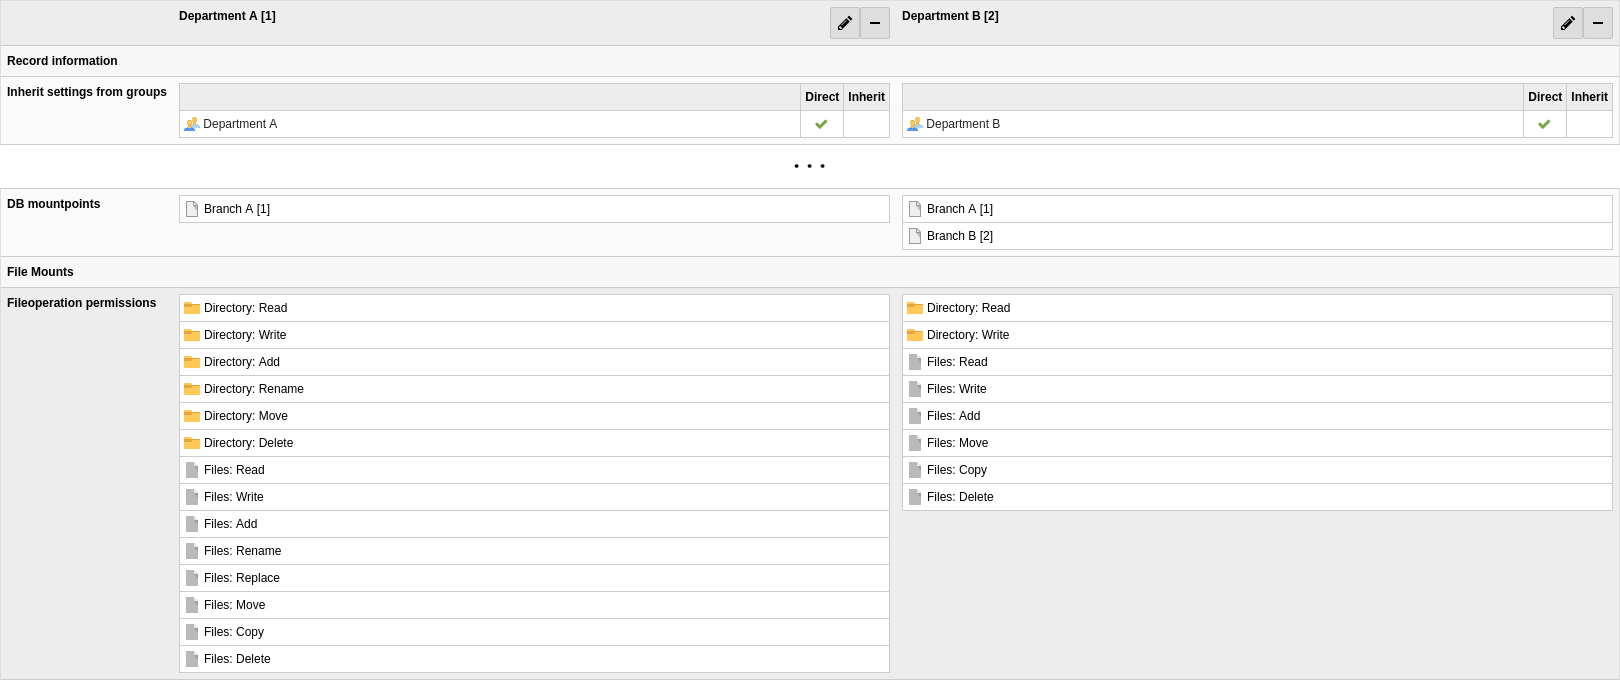
\includegraphics[width=0.9\linewidth]{ChangesForIntegrators/90826-CompareBackendUsergroups.png}
	\end{figure}

\end{frame}

% ------------------------------------------------------------------------------
% Important | 89555 | Workspace-related database records contain the proper Page ID

\begin{frame}[fragile]
	\frametitle{Changes for Integrators}
	\framesubtitle{Workspaces}

	\begin{itemize}
		\item For many years, the TYPO3 core set \texttt{pid} to \texttt{-1} of unpublished records.
		\item TYPO3 now handles versioned records by validating the following three fields:

			\begin{itemize}
				\item \texttt{t3ver\_wsid} (the workspace ID the record is versioned in)
				\item \texttt{t3ver\_state} (the type of the versioned record)
				\item \texttt{t3ver\_oid} (the live version of a record)
			\end{itemize}

		\item Therefore, \texttt{pid=-1} is not required anymore.
		\item The Upgrade Wizard converts all \texttt{pid} fields of versioned records
			into the real \texttt{pid} values.
		\item New installations are not affected by this change.

	\end{itemize}

\end{frame}

% ------------------------------------------------------------------------------
% Deprecation | 91030 | Runtime-Activated Packages

\begin{frame}[fragile]
	\frametitle{Changes for Integrators}
	\framesubtitle{Runtime-Activated Packages}

	\begin{itemize}
		\item The following global configuration option has been marked \textbf{deprecated}:\newline
			\smaller
				\texttt{\$GLOBALS['TYPO3\_CONF\_VARS']['EXT']['runtimeActivatedPackages']}
			\normalsize
		\item The use of runtime-activated extensions slows down a TYPO3 instance significantly.
		\item Integrators are adviced to take necessary steps, if such warnings apear
			in the deprecation log:\newline
			\begingroup
				\fontsize{8}{10}
				\texttt{Support for runtime activated packages will be removed in TYPO3 v11.0.}
			\endgroup

	\end{itemize}

\end{frame}

% ------------------------------------------------------------------------------
